%=============================================================================
% EXPERIMENTS AND RESULTS
% Order follows the CS3631 brief: comparative analysis, ablation, hyperparameter
% tuning, computational analysis, then the other experiments.
%
% EXP-062 (week-index fix) is PENDING. When it lands, the numbers that read a
% date-joined input change: B, the seasonal-feature and climate levers, and the
% nine-origin rows of tab:nine. Rebuild tables_generated.tex and re-check every
% number marked "EXP-062" below before submission.
%=============================================================================
\section{Experiments and Results}
\label{sec:experiments}

All numbers are RMSE in weekly cases on the corrected dataset. Sections
\ref{sec:comparative}--\ref{sec:compute} and
\ref{sec:seirgnn}--\ref{sec:valtest} come from the 810 runs of the reproduction
notebook; \S\ref{sec:prospective} comes from the prospective study. Validation decides
and test is reported beside it.

\subsection{Comparative analysis}
\label{sec:comparative}
Table~\ref{tab:encoders} compares every encoder and baseline on identical windows,
folds, loss, early stopping and metric, and Table~\ref{tab:paired} pairs \model{}
against the published head and against persistence.

\textbf{As published, three of five ST-GNNs fail.} Behind the direct head AAGCN,
ASTGCN and the LSTM score 16.71, 16.83 and 16.91 on validation, a spread of 0.20, and
all beat persistence (17.86). STGAT, A3TGCN and DCRNN score 22.93, 28.63 and 34.64,
worse than persistence by 5--17. They are underfitting rather than short of
information: a linear model fitted to their training residuals recovers 48\% and
60\% of STGAT's and A3TGCN's validation residual variance, against 3--7\% for the
working encoders.

\textbf{\model{} makes every encoder usable.} With \model{} all six encoders score
16.57--18.35 on validation and 33.53--39.02 on test. It repairs the three failing
encoders by 5.95, 10.95 and 16.29 on validation and 25.54, 23.24 and 34.50 on test, on
9/9 paired runs each ($\padj=0.004$). On the working encoders it changes validation by
at most 0.14 and improves AAGCN's test RMSE on 9/9 runs ($-1.62$).

\textbf{Against persistence, the strong encoders win.} AAGCN with \model{} beats
persistence on all 9 runs on validation ($-1.29$) and on test ($-2.48$), and ASTGCN
on 9/9 and 8/9 ($-1.10$, $-1.26$). The repaired encoders reach persistence but do not
go clearly beyond it, and DCRNN with \model{} stays slightly worse (+0.50). The
anchor removes failure; it cannot add information the encoder does not have.

\textbf{Baselines.} The graph adds little: a GCN beats the same network without
message passing by 0.06 (3/9, Table~\ref{tab:levers}). $k$-NN analogues, with no
network, reach 16.52 / 34.34; gradient-boosted trees reach 17.94, or 17.40 with
climate. The configuration validation selects, $B$ (AAGCN, direct head, NB loss,
seasonal features; 15.51), is worse than persistence on test (37.54). AAGCN with
\model{} has the lowest test RMSE of every configuration trained on the three origins
(33.53), but validation
would not have chosen it, so we report it as observed rather than selected.
% EXP-062: B, seasonal features and climate rows change after the week-index fix.

\subsection{Ablation study}
\label{sec:ablation}
Table~\ref{tab:rescue} builds \model{} from the published head one component at a
time: the persistence anchor (residual head), then the gate (\model{}), then the SEIR
branch. A pre-registered rule credits physics only if the SEIR branch beats \model{}
on at least 7 of 9 runs with $\padj<0.05$ on each failing encoder.

\textbf{The anchor removes the failure.} A residual head, with no gate, already brings
the failing encoders to 17.47--17.85. \textbf{The gate} improves on it for STGAT
(17.85 to 16.98), AAGCN and ASTGCN, and costs A3TGCN 0.21 and DCRNN 0.83; on the
prospective weeks it beats the ungated head ($-0.31$ [$-0.77$, $-0.08$],
Table~\ref{tab:prospective}). Anchor and gate together account for 96--112\% of the
repair that the full SEIR head achieves on each failing encoder.

\textbf{The SEIR branch adds nothing.} Added to \model{}, the simulator earns credit on
none of the three failing encoders: it is significantly \emph{worse} on STGAT ($+0.66$,
1/9, $\padj=0.023$), ties on A3TGCN ($-0.00$, 6/9), and helps DCRNN on only 3/9 runs.
On the working encoders it costs 0.75--0.86 (0 or 1 of 9 runs). On test the sign
reverses for the failing encoders (up to $-3.50$, 9/9); this was not used to decide
and is the validation--test disagreement of \S\ref{sec:valtest}.

\textbf{Why the pure SEIR decoder fails.} Routing the forecast entirely through the
simulator scores 24.01--25.75, worse than persistence on every encoder and 7.3--7.4
worse than the direct head on each working one. Inverting the simulator for the force
of infection that reproduces each observed count shows why: with transmission off, the
exposed state seeded from recent cases still emits \emph{more} cases than observed for
14--16\% of training targets, which no network output can reach; the required force of
infection is only $r^2=0.22$--$0.26$ predictable from case history, against
0.81--0.82 for the direct target; and susceptible depletion is not the cause (0.7--4.9\%
of cells reach the clamp).

\textbf{Loss and other levers.} Table~\ref{tab:levers} and Figure~\ref{fig:levers}
pair every further lever against its own control. The NB likelihood is the largest
controlled validation gain ($-0.76$, 9/9, $\padj=0.014$), larger than any architecture
change, because it corrects the median--mean bias of \S\ref{sec:loss}; on test it is
1.61 worse, so we do not adopt it in \model{}. No architecture change improves
validation by more than 0.15, and the literature's remedies are neutral or worse:
RevIN $+1.47$ (0/9), an STID-style MLP $+0.84$ (0/9), TimeGAN augmentation $+0.60$
(0/9), climate at lags 2--25 $+0.47$ (0/9).
% EXP-062: the seasonal-feature and climate lever rows change after the week-index fix.

\begin{figure}[t]
  \centering
  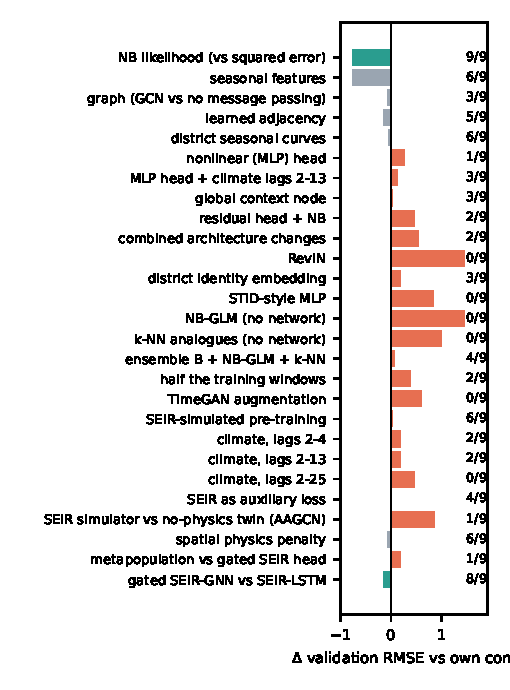
\includegraphics[width=\linewidth]{figures/fig_levers}
  \caption{Every lever's validation difference against its own control
  (Table~\ref{tab:levers}); win counts on the right. Green: negative and
  $\ge$7/9 wins. Grey: negative but inconsistent. Red: worse.}
  \label{fig:levers}
\end{figure}

\subsection{Hyperparameter tuning}
\label{sec:tuning}
In the main study every encoder and head uses the same fixed settings
(\S\ref{sec:impl}), chosen before the runs, so no model gets more tuning than another.
Before the prospective test we tuned each learned arm on the same grid and budget:
learning rate $\{10^{-3},3\times10^{-3}\}\times$ hidden size $\{32,64\}$, 108 runs per
arm on the nine development origins, selected on validation only. All three arms select
learning rate $3\times10^{-3}$ and $d=64$, the settings of the main study
(Table~\ref{tab:tuning}). The whole grid moves validation RMSE by at most 0.57, and the
ridge penalty of AR(3) by 0.12, so the conclusions do not hinge on tuning. Halving the
training windows costs $B$ 0.39 and a quarter of them 0.25 (Table~\ref{tab:levers}):
the models are not short of data.

\subsection{Computational analysis}
\label{sec:compute}
Table~\ref{tab:compute} gives the cost of each encoder and head. \model{} adds one
parameter and no measurable time per epoch (AAGCN 0.19 to 0.20 s). The SEIR branch adds
five parameters but roughly doubles the time per epoch on the light encoders (AAGCN
0.19 to 0.41 s), because it steps the simulator daily within every forecast week. The
encoders span three orders of magnitude, from AAGCN (2{,}873 parameters, 19 s per run)
to DCRNN (827{,}843 parameters, 3.6--4.1 s per epoch), and the smallest is the most
accurate. Every model trains on a free CPU; the full 810-run study takes 3.0 hours.

\subsection{Prospective evaluation, 2024--2026}
\label{sec:prospective}
The real test is weeks no setting was chosen on. We froze six arms and their settings
on development data, then parsed the new weeks (\S\ref{sec:newweeks}) and scored each
arm once on 85 forecast starts. The neural arms share one encoder, a Graph
WaveNet-style network with a learned adjacency~\cite{wu2019graphwavenet}, the
development finalist: \model{}, \model{} with the SEIR branch (the pre-registered
proposed model), and the residual head. Persistence, seasonal naive and an AR(3)
ridge regression complete the list.

Table~\ref{tab:prospective} gives the result. \textbf{No learned model beats
persistence on RMSE}: persistence scores 34.75, \model{} 35.43 and \model{}+SEIR 35.40,
differences that are not significant (\model{}+SEIR $+0.65$, $p_{\text{Holm}}=0.62$).
\textbf{The SEIR branch adds nothing} over \model{} ($-0.03$ [$-0.41$, $+0.12$],
$p_{\text{Holm}}=0.67$). On the secondary metrics the learned arms do better than
persistence (MAE 11.35 against 11.78, SMAPE 45.7 against 50.3), and every arm beats the
seasonal naive forecast by 26--28 RMSE. RMSE is dominated by the 2026 outbreak:
persistence scores 14.72, 20.05 and 160.51 in 2024, 2025 and 2026, and \model{} 14.32,
21.43 and 162.75. \model{} is better in the quiet year and worse in the outbreak, where
the next large move is not in the inputs. The development advantage of the SEIR arm over
persistence (27.34 against 28.54) does not carry over to later data.

Because the SEIR branch ties its no-SEIR twin, we present the simpler \model{} as the
framework. That choice is made after seeing the prospective result, and we state it as
such: the pre-registered finalist was the SEIR variant, and the two are equivalent.

\subsection{SEIR-GNN against SEIR-LSTM, and physics as structure}
\label{sec:seirgnn}
Behind the same gated SEIR head the graph beats the LSTM on three origins on
validation (ASTGCN $-0.54$, 9/9; AAGCN $-0.14$, 8/9), but on nine disjoint origins the
advantage is not robust to the encoder or the metric (Table~\ref{tab:nine}): ASTGCN's
holds on validation ($-0.62$, 8/9, $p=0.012$) and vanishes on test, and AAGCN's reverses.
Two further physics structures do not help: a spatial penalty on relative incidence
across borders ($-0.06$, 6/9) and a metapopulation SEIR head that couples districts
inside the dynamics ($+0.20$ against the gated SEIR head, 1/9, $\padj=0.020$). The data
explain why: on the district graph, Moran's $I$ is 0.29 for log cases but $-0.03$ for
weekly log growth, so levels cluster in space while changes in transmission do not.
% EXP-062: the nine-origin rows of tab:nine change after the week-index fix.

\subsection{The ceiling is informational}
\label{sec:ceiling}
The working encoders, the SEIR-LSTM and $k$-NN, which has no network and no training,
leave residuals that correlate 0.91--0.97 with $B$'s: the models make the same errors.
The remaining error is a lag on moves. $B$ under-predicts rising weeks by 11.5 cases and
over-predicts falling weeks by 10.1, and the top 5\% of district-weeks carry 54--67\% of
every model's squared error. That is what a mean-seeking objective produces on a
near-random-walk target whose next move is not in the inputs.

\subsection{Validation and test disagree, systematically}
\label{sec:valtest}
Across the eight families of runs, the configuration validation selects is worse than
persistence on test in five, and the best configuration on test is anchored to the
last observation in six (\model{}, residual, gated SEIR or $k$-NN). A 30-week validation
span immediately before each origin appears to reward fitting that span's level, which
does not carry into the next period. This is one reason we report the prospective test
as the decisive evidence.
